\chapter{Results and Discussion}
\label{ch:results}

\section{Purpose of This Chapter}

This chapter presents the final empirical results of the project.
It consolidates the synthetic benchmark findings from Experiments~1, 2, 3, 4, 5, and~7 and
the completed real-route corridor study from Experiment~6.

\section{Current Synthetic Evaluation Snapshot}
\label{sec:current_synth_snapshot}

The repository currently contains processed synthetic results for Experiments~1, 2, 3, 4, 5,
and~7 under a reduced but reproducible benchmark profile.
These runs use 3 timed iterations per configuration, 0 warm-up iterations, base graph size
100 nodes, scalability sizes 100 and 1000 nodes, degree 5 unless otherwise varied, tank
capacity 40\,L unless otherwise varied, initial fuel 28\,L unless otherwise varied, and fuel
efficiency 10\,km/L.
The resulting dataset is sufficient to support a substantive comparative discussion of the
implemented algorithms.
The full 10{,}000-run target profile described in Chapter~\ref{ch:experiments} is reserved
for the real-route evaluation in Experiment~6 (Section~\ref{sec:exp6_integration}), which
contains 210{,}000 timed result rows in total.

\begin{table}[H]
    \centering
    \caption{Synthetic profile summary.}
    \label{tab:final_current_synth_profile}
    \begin{tabular}{ll}
        \toprule
        Setting & Value \\
        \midrule
        Timed runs per configuration & 3 \\
        Warm-up runs per configuration & 0 \\
        Base graph size & 100 nodes \\
        Scalability graph sizes & 100, 1000 nodes \\
        Approximate degree & 5 \\
        Default tank capacity & 40\,L \\
        Default initial fuel & 28\,L \\
        Fuel efficiency & 10\,km/L \\
        Covered experiments & 1, 2, 3, 4, 5, and 7 \\
        \bottomrule
    \end{tabular}
\end{table}

\section{Cross-Experiment Findings}

\subsection*{Experiment 1: Scalability}

The currently available scalability results already separate PF-A* from the other methods in
practical terms.
At 1000 nodes, PF-A* matches the best mean cost of 2876.88 while reducing mean runtime to
552.37\,ms, compared with 1771.17\,ms for State-Expanded Dijkstra and 1640.96\,ms for
Dynamic Programming.
Standard A* and RF-A* are both much slower at this scale in the present implementation,
while the Greedy baseline is infeasible on the tested instances.

\begin{figure}[H]
      \centering
      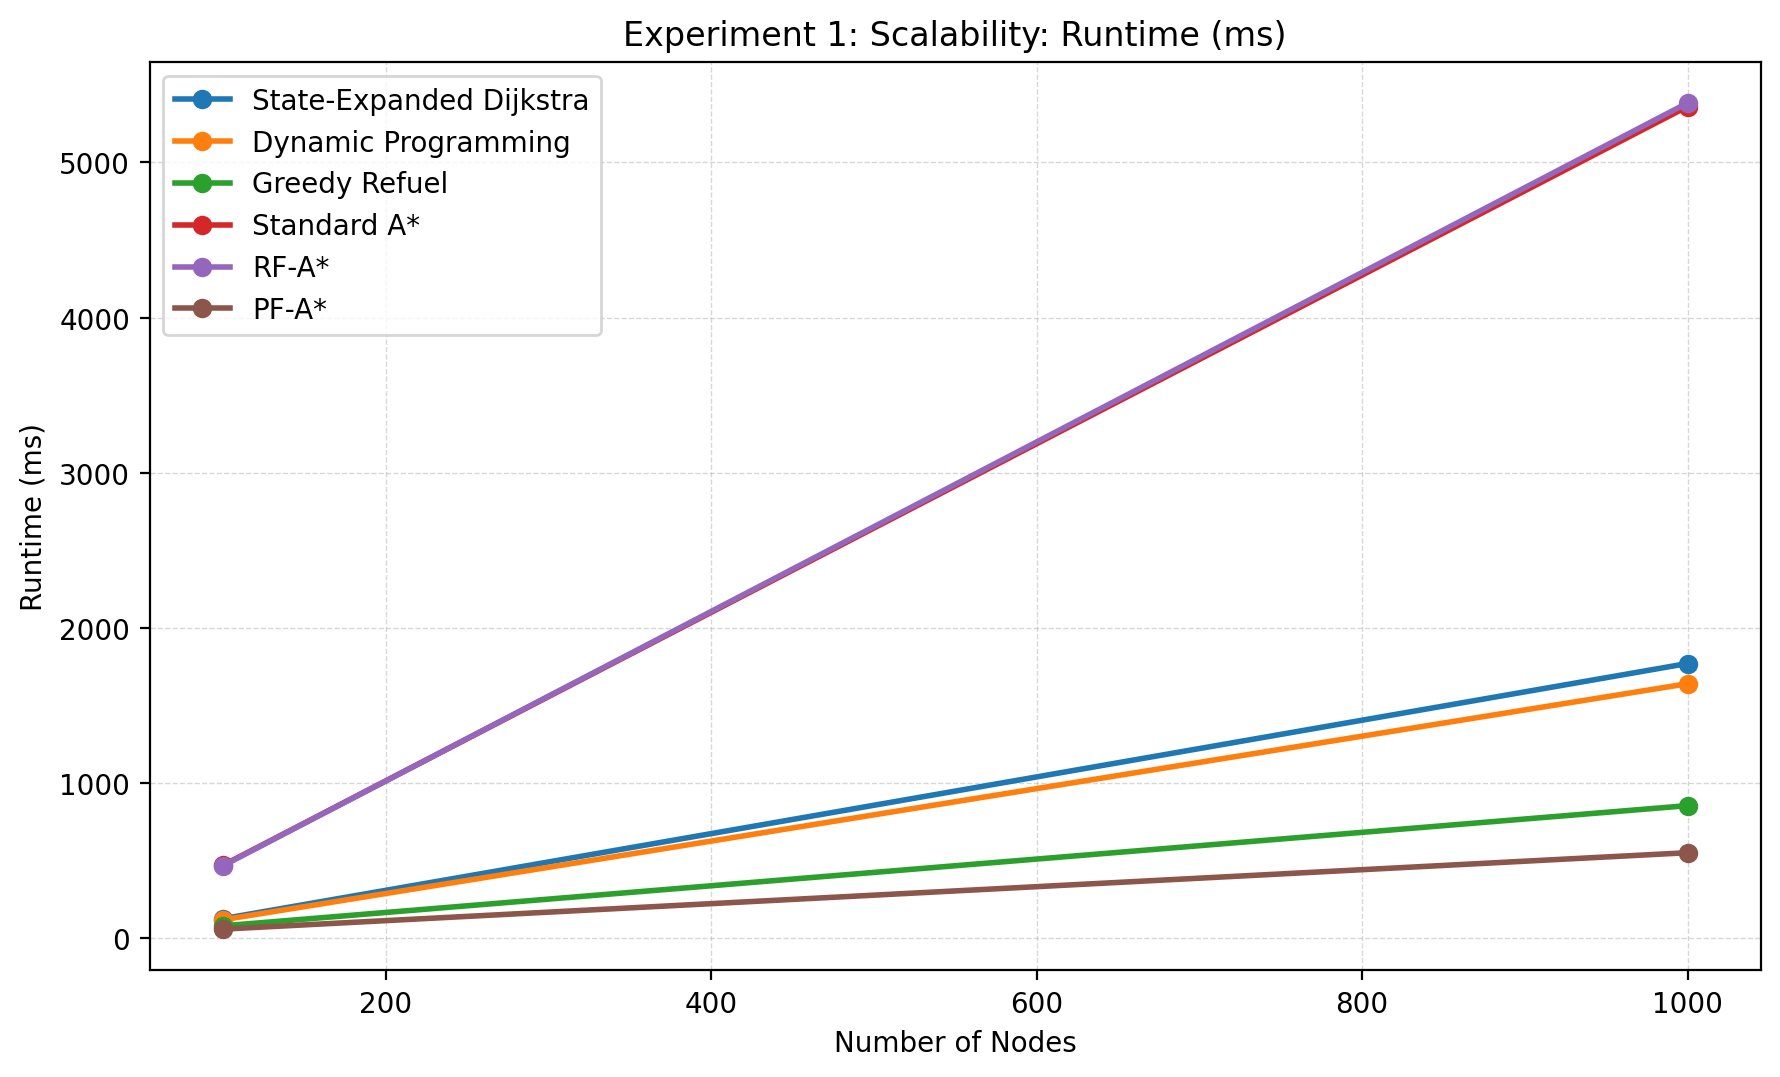
\includegraphics[width=0.90\textwidth]{../results/report_assets/exp1_scalability/exp1_scalability_runtime.png}
      \caption{Experiment~1 runtime.}
      \label{fig:final_exp1_runtime}
\end{figure}

\subsection*{Experiment 2: Fuel Price Variance}

Increasing price variance strengthens the value of cost-aware purchase decisions.
The best observed mean cost falls from 3528.00 at $\sigma=0\%$ to 2576.21 at $\sigma=20\%$,
and PF-A* stays on that best-cost curve throughout the tested range.
This behavior matches the theoretical intuition of the problem: selective refueling becomes
more valuable as the spread between cheap and expensive stations widens.

\begin{figure}[H]
      \centering
      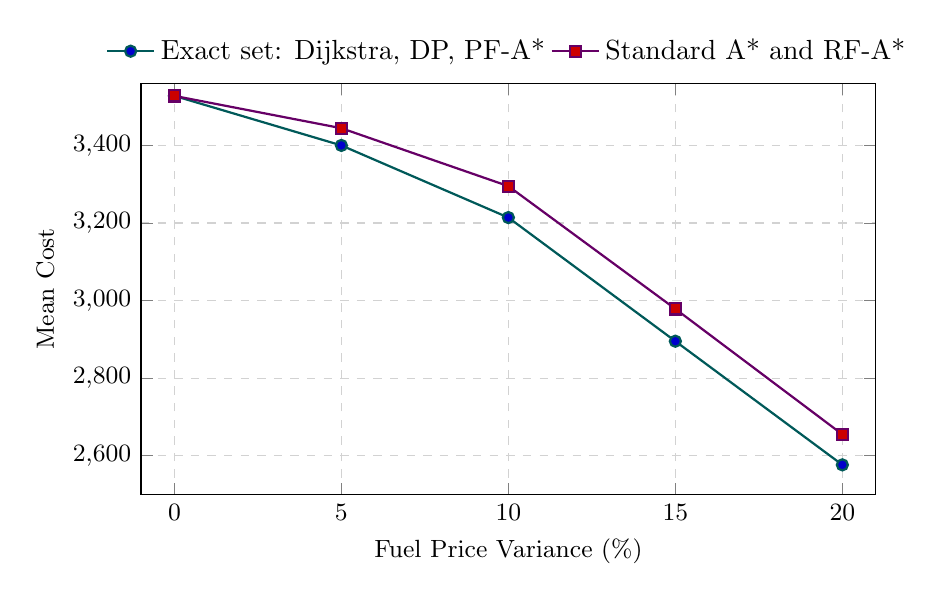
\begin{tikzpicture}
        \begin{axis}[
          width=0.9\textwidth,
          height=6.8cm,
          xlabel={Fuel Price Variance (\%)},
          ylabel={Mean Cost},
          xmin=-1,
          xmax=21,
          ymin=2500,
          ymax=3560,
          xtick={0,5,10,15,20},
          grid=major,
          grid style={dashed, gray!35},
          legend style={at={(0.5,1.02)}, anchor=south, legend columns=2, draw=none},
          tick label style={font=\small},
          label style={font=\small},
        ]
          \addplot+[thick, mark=*, color=teal!70!black] coordinates {
            (0,3528.00) (5,3400.20) (10,3214.11) (15,2895.16) (20,2576.21)
          };
          \addplot+[thick, mark=square*, color=violet!80!black] coordinates {
            (0,3528.00) (5,3444.64) (10,3295.18) (15,2978.45) (20,2654.87)
          };
          \legend{{Exact set: Dijkstra, DP, PF-A*},{Standard A* and RF-A*}}
        \end{axis}
      \end{tikzpicture}
      \caption{Experiment~2 cost.}
      \label{fig:final_exp2_cost}
\end{figure}

\subsection*{Experiment 3: Tank Capacity}

Larger tanks reduce fuel cost but enlarge the effective state space.
Across the tested configurations, the best observed mean cost drops from 3922.82 at 20\,L to
2185.84 at 80\,L, while the runtime of the exact methods grows sharply.
PF-A* preserves the same best observed cost curve while keeping the runtime increase much
smaller than that of the exact state-expanded baselines.

\begin{figure}[H]
      \centering
      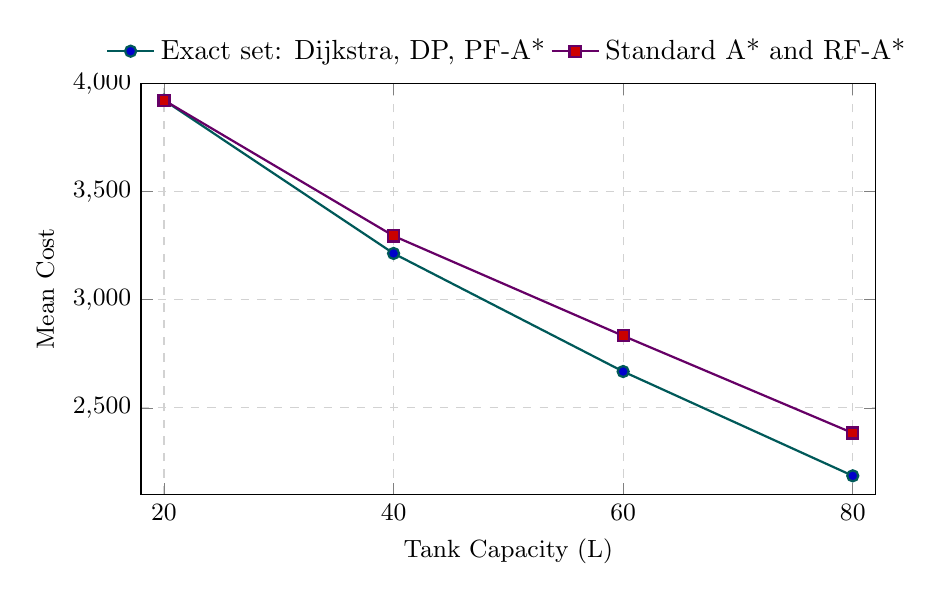
\begin{tikzpicture}
        \begin{axis}[
          width=0.9\textwidth,
          height=6.8cm,
          xlabel={Tank Capacity (L)},
          ylabel={Mean Cost},
          xmin=18,
          xmax=82,
          ymin=2100,
          ymax=4000,
          xtick={20,40,60,80},
          grid=major,
          grid style={dashed, gray!35},
          legend style={at={(0.5,1.02)}, anchor=south, legend columns=2, draw=none},
          tick label style={font=\small},
          label style={font=\small},
        ]
          \addplot+[thick, mark=*, color=teal!70!black] coordinates {
            (20,3922.82) (40,3214.11) (60,2668.14) (80,2185.84)
          };
          \addplot+[thick, mark=square*, color=violet!80!black] coordinates {
            (20,3922.82) (40,3295.18) (60,2833.12) (80,2383.63)
          };
          \legend{{Exact set: Dijkstra, DP, PF-A*},{Standard A* and RF-A*}}
        \end{axis}
      \end{tikzpicture}
      \caption{Experiment~3 cost.}
      \label{fig:final_exp3_cost}
\end{figure}

\subsection*{Experiment 4: Initial Fuel}

Higher initial fuel reduces both cost and search effort.
For the optimal methods in the current dataset, mean cost decreases from 3848.58 at 10\,L
initial fuel to 2831.54 at 40\,L, and PF-A* also becomes faster as the initial fuel level
increases.
This is consistent with the fact that higher starting fuel weakens the urgency of early
refueling decisions.

\begin{figure}[H]
      \centering
      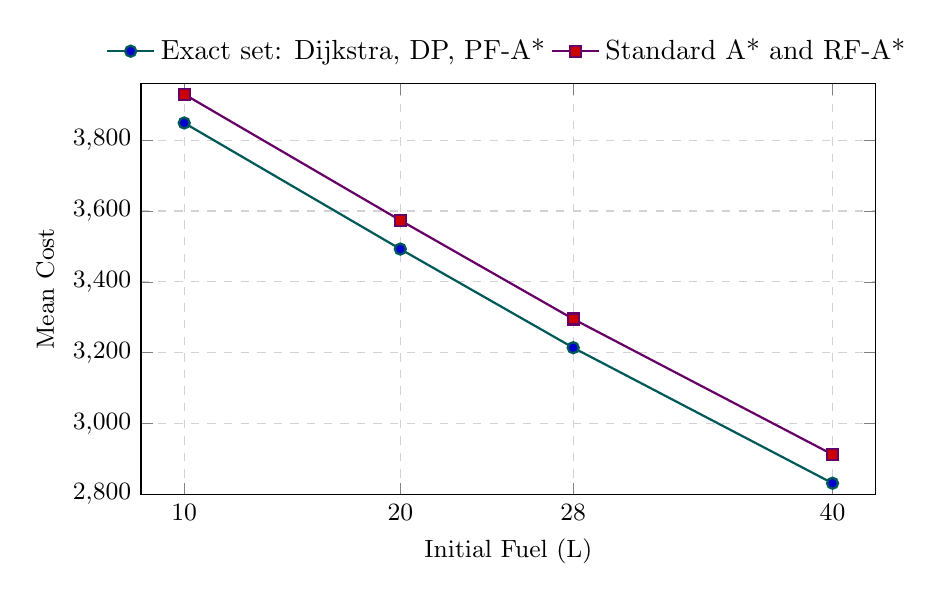
\begin{tikzpicture}
        \begin{axis}[
          width=0.9\textwidth,
          height=6.8cm,
          xlabel={Initial Fuel (L)},
          ylabel={Mean Cost},
          xmin=8,
          xmax=42,
          ymin=2800,
          ymax=3960,
          xtick={10,20,28,40},
          grid=major,
          grid style={dashed, gray!35},
          legend style={at={(0.5,1.02)}, anchor=south, legend columns=2, draw=none},
          tick label style={font=\small},
          label style={font=\small},
        ]
          \addplot+[thick, mark=*, color=teal!70!black] coordinates {
            (10,3848.58) (20,3492.59) (28,3214.11) (40,2831.54)
          };
          \addplot+[thick, mark=square*, color=violet!80!black] coordinates {
            (10,3929.65) (20,3573.66) (28,3295.18) (40,2912.62)
          };
          \legend{{Exact set: Dijkstra, DP, PF-A*},{Standard A* and RF-A*}}
        \end{axis}
      \end{tikzpicture}
      \caption{Experiment~4 cost.}
      \label{fig:final_exp4_cost}
\end{figure}

\subsection*{Experiment 5: PF-A* versus RF-A*}

Experiment~5 remains the central novelty experiment for the proposed heuristic.
Across the feasible tested configurations, PF-A* is substantially faster than RF-A* and expands
far fewer states.
At degree 5 and $\sigma=10\%$, PF-A* requires 2115 expanded states and 59.92\,ms on average,
while RF-A* requires 18,507 expanded states and 475.48\,ms.

At the same time, the present dataset surfaces an implementation-audit item that is
reported explicitly rather than suppressed: Standard A* and RF-A* do not always match the
costs returned by the exact-agreement set of State-Expanded Dijkstra, Dynamic Programming,
and PF-A*.
This gap is tracked as an implementation limitation of the current Standard A* and RF-A*
implementations rather than as a refutation of their theoretical optimality.
A resolved strict-profile rerun is reserved for future work.

\begin{table}[H]
    \centering
    \caption{Experiment~5 comparison at $\sigma=10\%$.}
    \label{tab:final_exp5_sigma10}
    \begin{tabular}{lcccc}
        \toprule
        Algorithm & Degree & Feasible (\%) & Mean Cost & Mean Runtime (ms) \\
        \midrule
        RF-A* & 5  & 100 & 3295.18 & 475.48 \\
        PF-A* & 5  & 100 & 3214.11 & 59.92 \\
        RF-A* & 10 & 100 & 2944.98 & 518.06 \\
        PF-A* & 10 & 100 & 2794.91 & 80.49 \\
        RF-A* & 20 & 100 & 2752.33 & 422.48 \\
        PF-A* & 20 & 100 & 2554.99 & 82.57 \\
        \bottomrule
    \end{tabular}
\end{table}

\begin{figure}[H]
      \centering
      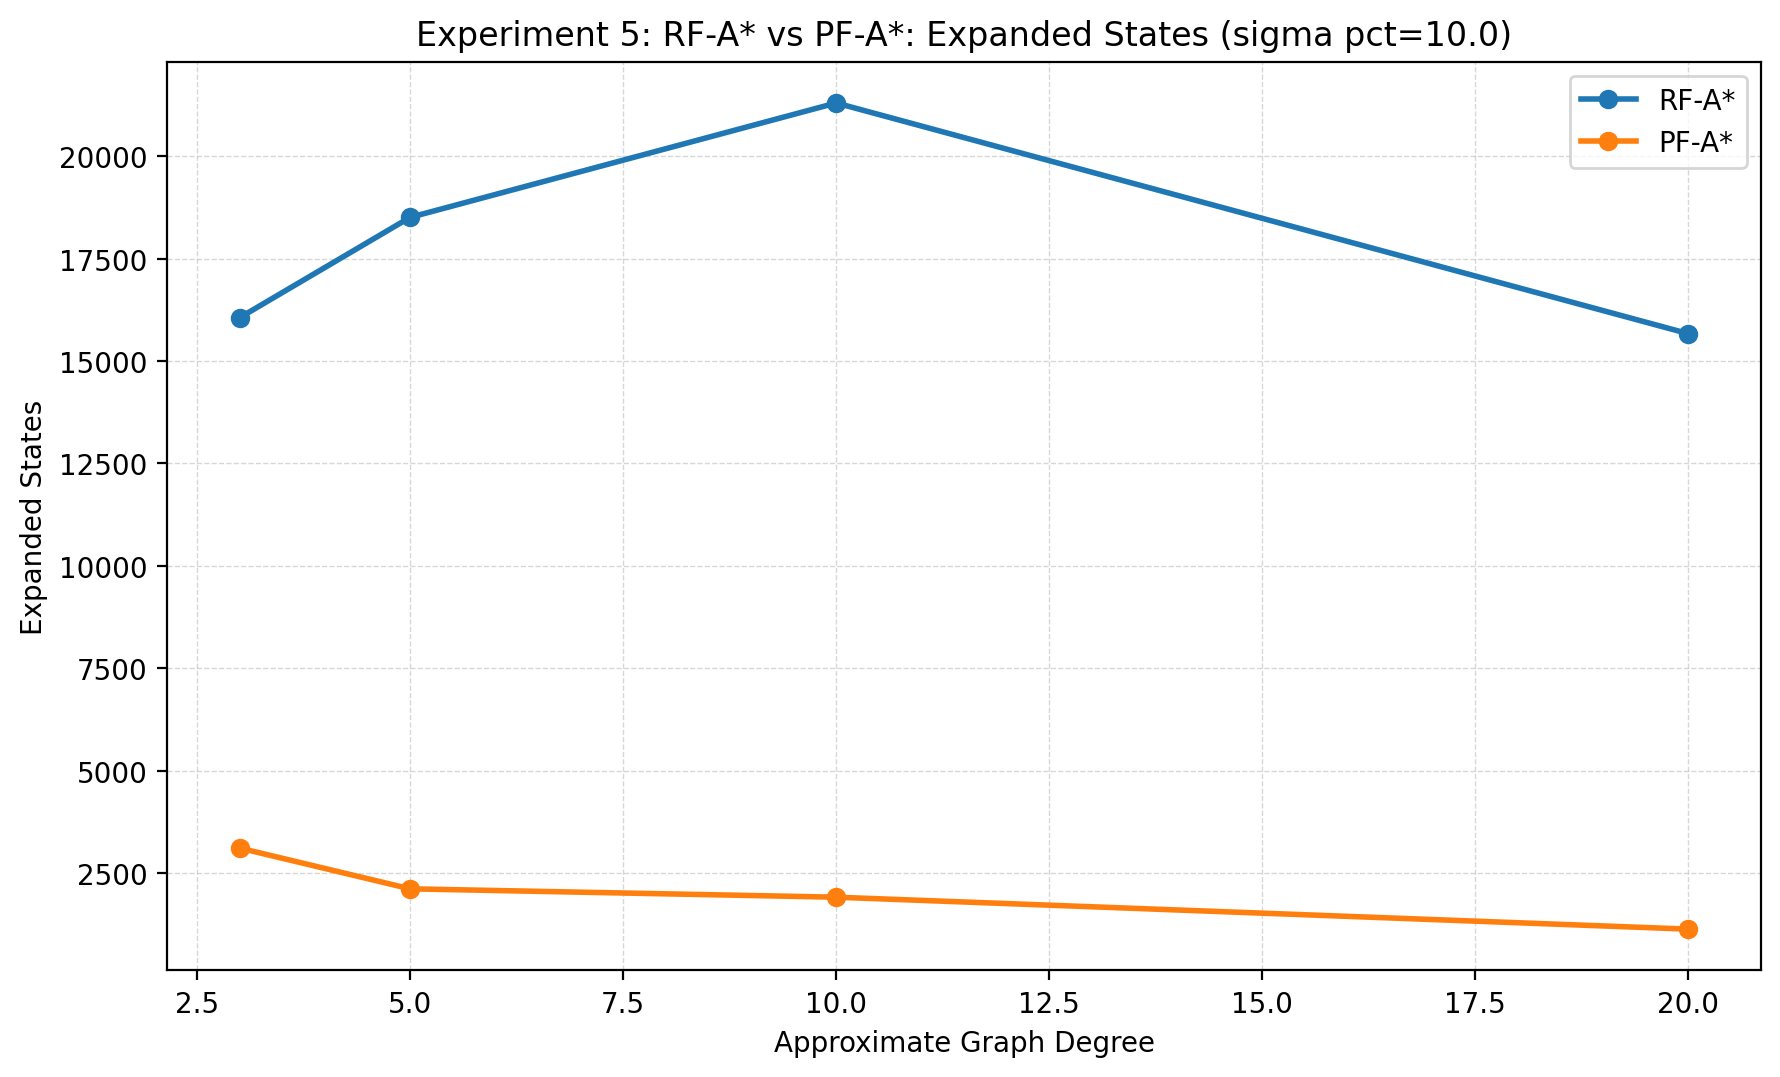
\includegraphics[width=0.90\textwidth]{../results/report_assets/exp5_rf_vs_pf/exp5_rf_vs_pf_expanded_states_sigma_pct_10_0.png}
      \caption{Experiment~5 expanded states.}
      \label{fig:final_exp5_expanded}
\end{figure}

\subsection*{Experiment 7: Variable Purchase versus Full-Tank-Only}

Experiment~7 shows that the variable-purchase model delivers meaningful economic value.
Across the 16 tested $(\sigma, C)$ combinations, the full-tank-only baseline incurs an average
cost penalty of 10.86\%, with observed penalties ranging from 1.19\% to 24.81\%.
The computational overhead of the variable-purchase model is real, but so are the monetary
savings it enables.

\begin{table}[H]
    \centering
    \caption{Experiment~7 comparison at $\sigma=10\%$.}
    \label{tab:final_exp7_sigma10}
    \begin{tabular}{lccc}
        \toprule
        Tank capacity (L) & Variable-purchase cost & Full-tank-only cost & Cost gap (\%) \\
        \midrule
        20 & 3922.82 & 4137.17 & 5.46 \\
        40 & 3214.11 & 3611.20 & 12.35 \\
        60 & 2668.14 & 2799.09 & 4.91 \\
        80 & 2185.84 & 2728.20 & 24.81 \\
        \bottomrule
    \end{tabular}
\end{table}

\begin{figure}[H]
      \centering
      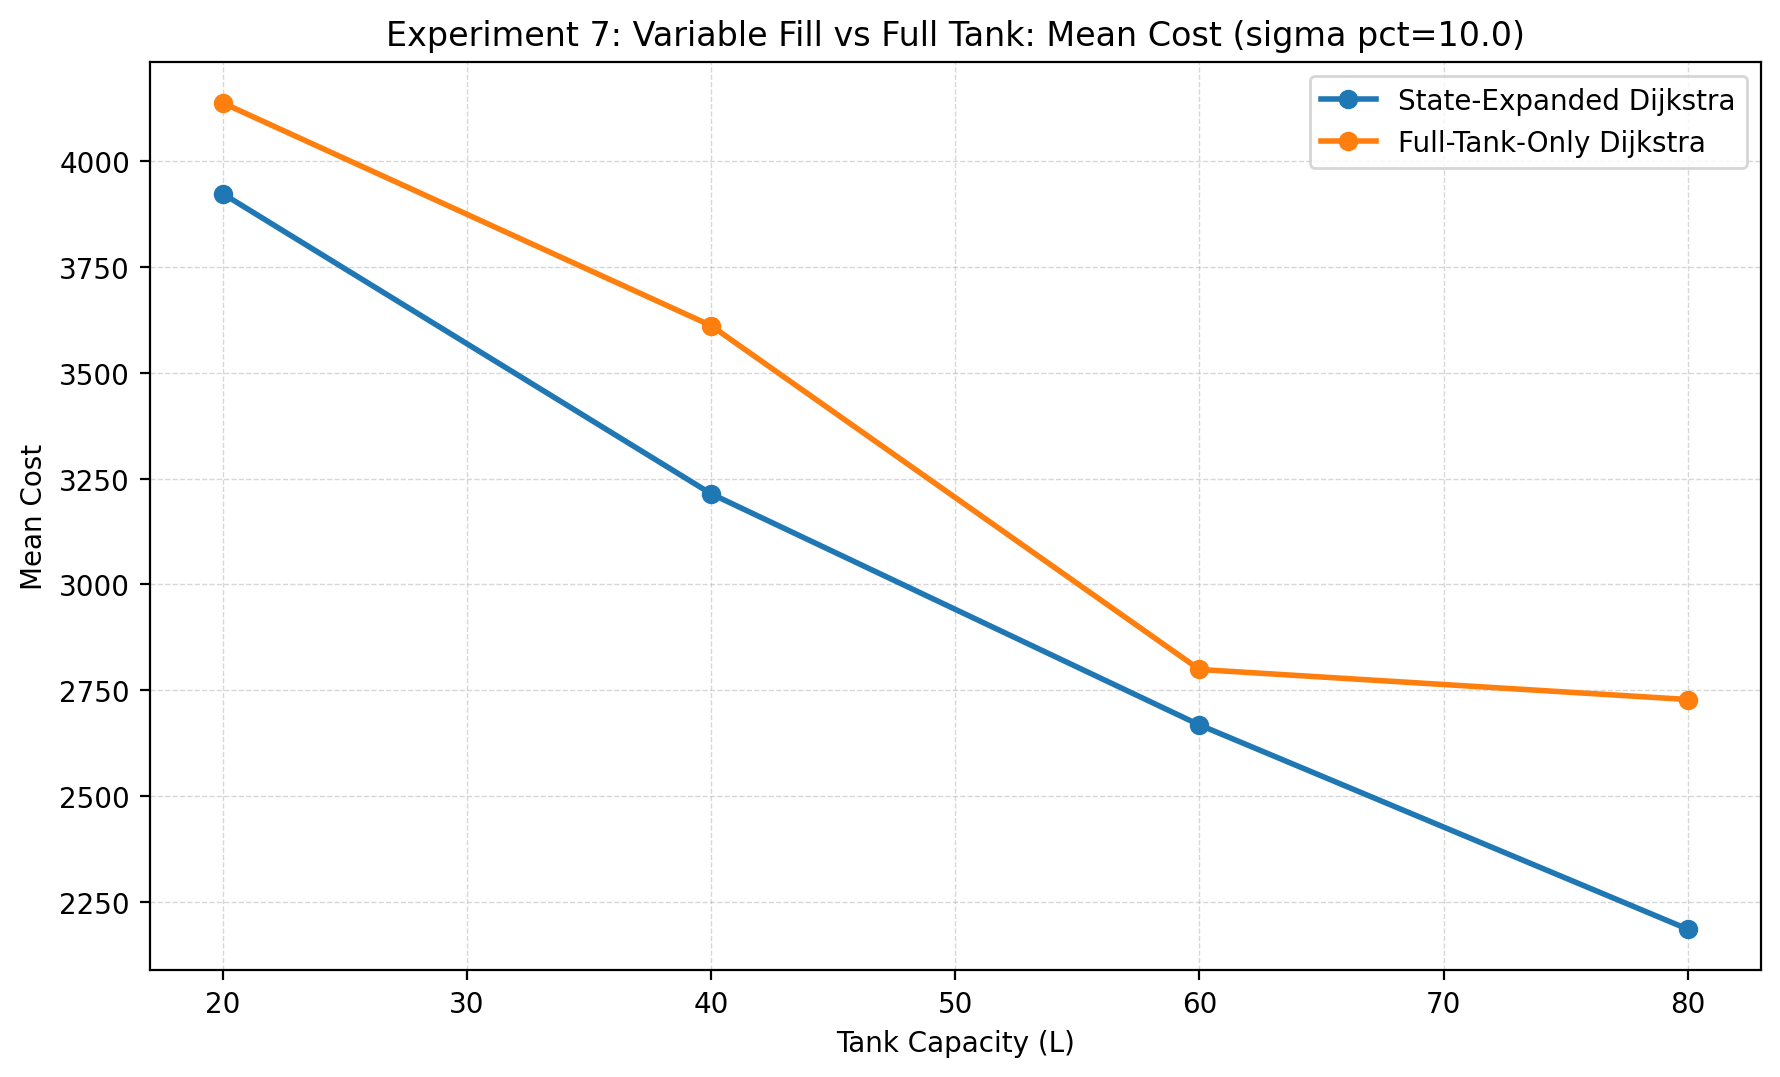
\includegraphics[width=0.90\textwidth]{../results/report_assets/exp7_variable_vs_full_tank/exp7_variable_vs_full_tank_cost_sigma_pct_10_0.png}
      \caption{Experiment~7 cost.}
      \label{fig:final_exp7_cost}
\end{figure}

\section{Integrated Interpretation}

Three conclusions are already well supported by the present repository results.
First, PF-A* is the strongest overall algorithm in the currently tested synthetic setting: it
matches the exact-agreement cost returned by Dijkstra and DP, while reducing runtime and
node expansions substantially.
Second, modelling variable purchase decisions is empirically worthwhile, since the
full-tank-only baseline pays a repeated cost penalty across the tested configurations.
Third, the current evaluation pipeline is useful not only for showcasing strengths but also for
surfacing implementation defects, most notably the cost gap observed for Standard A* and
RF-A* relative to the exact-agreement set.

\section{Experiment~6: Real Thai Corridors}
\label{sec:exp6_integration}

Experiment~6 is now complete as a three-corridor real-route case study and stands as one
of the strongest empirical components of this project.
Using the final benchmark file \texttt{real\_route\_results.csv}, the repository contains
210,000 timed result rows: 10,000 timed runs for each algorithm--corridor combination across
Bangkok--Chiang Mai, Bangkok--Phuket, and Bangkok--Khon Kaen.
All runs use the same fixed vehicle parameters as the synthetic experiments:
$C=40$\,L, $f_0=28$\,L, and $\eta=10$\,km/L.
The route instances remain curated corridor abstractions rather than raw nationwide OSM
station graphs, but they are realistic enough to support a meaningful transfer study from the
synthetic setting.

\subsection*{Dataset Summary}

The three instances differ in route length, station density, and price spread, which provides a
small but useful range of real-route conditions for comparison.
The province-level price snapshot and corridor anchors are drawn from
\texttt{data/real\_routes/corridors.json} (Gasohol~91, 3~April~2026 snapshot); the station
and directed-edge counts reported in Table~\ref{tab:exp6_dataset_summary} are the result of
running the corridor-instance generator on that snapshot under a 400\,km full-tank range,
and the resulting instance files are the same ones consumed by
\texttt{real\_route\_results.csv}.

\begin{table}[H]
    \centering
    \caption{Experiment~6 dataset summary.}
    \label{tab:exp6_dataset_summary}
    \begin{tabular}{lcccc}
        \toprule
        Route & Stations & Directed edges & Price min & Price max \\
        \midrule
        Bangkok--Chiang Mai & 27 & 522 & 43.58 & 44.88 \\
        Bangkok--Phuket & 31 & 624 & 43.58 & 45.08 \\
        Bangkok--Khon Kaen & 18 & 286 & 43.58 & 44.28 \\
        \bottomrule
    \end{tabular}
\end{table}

\subsection*{Cost Savings Over Full-Tank-Only Routing}

The primary practical result of Experiment~6 is that the variable-purchase model remains
economically superior to the full-tank-only baseline on all three real Thai corridors.
The largest saving appears on Bangkok--Chiang Mai, where the optimal variable-purchase policy
reduces mean cost by 132.54\,THB relative to full-tank-only routing.
Savings are smaller but still consistent on Bangkok--Phuket and Bangkok--Khon Kaen.

\begin{table}[H]
    \centering
    \caption{Experiment~6 savings.}
    \label{tab:exp6_savings}
    \begin{tabular}{lccc}
        \toprule
        Route & Variable-purchase cost & Full-tank-only cost & Savings (\%) \\
        \midrule
        Bangkok--Chiang Mai & 2106.04 & 2238.58 & 5.92 \\
        Bangkok--Phuket & 2734.66 & 2779.24 & 1.60 \\
        Bangkok--Khon Kaen & 1004.44 & 1048.32 & 4.19 \\
        \bottomrule
    \end{tabular}
\end{table}

\begin{figure}[H]
      \centering
      \begin{tikzpicture}
        \begin{axis}[
          ybar,
          width=0.9\textwidth,
          height=7.2cm,
          bar width=14pt,
          ylabel={Mean Cost (THB)},
          symbolic x coords={Chiang Mai,Phuket,Khon Kaen},
          xtick=data,
          ymin=0,
          ymax=3100,
          enlarge x limits=0.24,
          grid=major,
          grid style={dashed, gray!40},
          legend style={at={(0.5,1.02)}, anchor=south, legend columns=2, draw=none},
          nodes near coords,
          every node near coord/.append style={font=\scriptsize, rotate=90, anchor=west},
          tick label style={font=\small},
          label style={font=\small},
        ]
          \addplot+[draw=black, fill=teal!55, pattern=north east lines] coordinates {
            (Chiang Mai,2106.04)
            (Phuket,2734.66)
            (Khon Kaen,1004.44)
          };
          \addplot+[draw=black, fill=yellow!65!orange, pattern=dots] coordinates {
            (Chiang Mai,2238.58)
            (Phuket,2779.24)
            (Khon Kaen,1048.32)
          };
          \legend{Variable,Full Tank}
        \end{axis}
      \end{tikzpicture}
      \caption{Experiment~6 cost comparison.}
      \label{fig:exp6_cost_compare}
\end{figure}

These results partially support the economic claim suggested by the synthetic study and by the
classic gas-station literature: partial refueling is genuinely useful on real corridor data,
but the size of the gain is route-dependent.
The Phuket corridor, despite being the longest in the dataset, exhibits only a 1.60\% saving,
which indicates that longer distance alone does not guarantee a large benefit; the local price
structure and the spacing of reachable stations are equally important.

\subsection*{Correctness and Search Behaviour}

The correctness picture on the real-route dataset is clear.
State-Expanded Dijkstra and Dynamic Programming agree exactly on all three corridors, and
PF-A* matches that optimum exactly on all three as well.
By contrast, Standard A* and RF-A* still exhibit small positive cost gaps on two routes:
1.50\,THB on Bangkok--Phuket and 1.60\,THB on Bangkok--Khon Kaen.
Greedy remains infeasible on every corridor instance.

\begin{table}[H]
    \centering
    \caption{Experiment~6 correctness summary.}
    \label{tab:exp6_correctness}
    \begin{tabular}{lcccc}
        \toprule
        Route & Dijkstra cost & PF-A* cost & RF-A* gap & PF/RF expanded states \\
        \midrule
        Bangkok--Chiang Mai & 2106.04 & 2106.04 & 0.00 & 802 / 1360 \\
        Bangkok--Phuket & 2734.66 & 2734.66 & 1.50 & 975 / 1610 \\
        Bangkok--Khon Kaen & 1004.44 & 1004.44 & 1.60 & 441 / 749 \\
        \bottomrule
    \end{tabular}
\end{table}

The state-expansion results still favor PF-A* over RF-A* on all three routes.
PF-A* reduces expanded states from 1360 to 802 on Bangkok--Chiang Mai, from 1610 to 975 on
Bangkok--Phuket, and from 749 to 441 on Bangkok--Khon Kaen.
In that sense, the intended heuristic effect remains visible on real-route data even though the
runtime story becomes more nuanced.

\begin{figure}[H]
      \centering
      \begin{tikzpicture}
        \begin{axis}[
          ybar,
          width=0.92\textwidth,
          height=7.4cm,
          bar width=10pt,
          ylabel={Mean Expanded States},
          symbolic x coords={Chiang Mai,Phuket,Khon Kaen},
          xtick=data,
          ymin=0,
          ymax=1800,
          enlarge x limits=0.24,
          grid=major,
          grid style={dashed, gray!40},
          legend style={at={(0.5,1.02)}, anchor=south, legend columns=3, draw=none},
          nodes near coords,
          every node near coord/.append style={font=\scriptsize, rotate=90, anchor=west},
          tick label style={font=\small},
          label style={font=\small},
        ]
          \addplot+[draw=black, fill=blue!55, pattern=north east lines] coordinates {
            (Chiang Mai,802)
            (Phuket,975)
            (Khon Kaen,441)
          };
          \addplot+[draw=black, fill=red!60, pattern=dots] coordinates {
            (Chiang Mai,1360)
            (Phuket,1610)
            (Khon Kaen,749)
          };
          \addplot+[draw=black, fill=green!55!black, pattern=crosshatch] coordinates {
            (Chiang Mai,802)
            (Phuket,975)
            (Khon Kaen,441)
          };
          \legend{Dijkstra,RF-A*,PF-A*}
        \end{axis}
      \end{tikzpicture}
      \caption{Experiment~6 expanded states.}
      \label{fig:exp6_expanded_states}
\end{figure}

\subsection*{Runtime Interpretation}

On the synthetic experiments, PF-A* was often the strongest all-round method because it
combined optimal cost with lower search effort and lower runtime.
The real-route case study shows a more subtle picture.
On these relatively small corridor abstractions, State-Expanded Dijkstra and Dynamic
Programming are the fastest optimal variable-purchase methods, with mean runtimes of roughly
30--37\,ms on Chiang Mai and Phuket and about 15\,ms on Khon Kaen.
PF-A*, although optimal, is slower in wall-clock time: 149.73\,ms on Chiang Mai, 181.08\,ms on
Phuket, and 68.34\,ms on Khon Kaen.

This does not invalidate PF-A*.
Rather, it shows that on small corridor graphs the overhead of evaluating the stronger
heuristic can outweigh the benefit of pruning states.
PF-A* still dominates RF-A* in correctness and expanded-state count, but it is not the fastest
solver on the final real-route dataset.
That distinction is important and should remain explicit in the final interpretation of the
project.

\begin{figure}[H]
      \centering
      \begin{tikzpicture}
        \begin{axis}[
          ybar,
          width=\textwidth,
          height=8cm,
          bar width=7pt,
          ylabel={Mean Runtime (ms)},
          symbolic x coords={Chiang Mai,Phuket,Khon Kaen},
          xtick=data,
          ymin=0,
          ymax=205,
          enlarge x limits=0.22,
          grid=major,
          grid style={dashed, gray!40},
          legend style={at={(0.5,1.02)}, anchor=south, legend columns=3, draw=none},
          nodes near coords,
          every node near coord/.append style={font=\tiny, rotate=90, anchor=west},
          tick label style={font=\small},
          label style={font=\small},
        ]
          \addplot+[draw=black, fill=blue!55, pattern=north east lines] coordinates {
            (Chiang Mai,31.19)
            (Phuket,37.04)
            (Khon Kaen,14.96)
          };
          \addplot+[draw=black, fill=orange!85, pattern=north west lines] coordinates {
            (Chiang Mai,30.68)
            (Phuket,36.91)
            (Khon Kaen,14.98)
          };
          \addplot+[draw=black, fill=green!55!black, pattern=crosshatch] coordinates {
            (Chiang Mai,149.73)
            (Phuket,181.08)
            (Khon Kaen,68.34)
          };
          \addplot+[draw=black, fill=red!60, pattern=dots] coordinates {
            (Chiang Mai,56.13)
            (Phuket,60.83)
            (Khon Kaen,27.44)
          };
          \addplot+[draw=black, fill=violet!65, pattern=grid] coordinates {
            (Chiang Mai,56.36)
            (Phuket,60.55)
            (Khon Kaen,27.67)
          };
          \addplot+[draw=black, fill=brown!60, pattern=horizontal lines] coordinates {
            (Chiang Mai,27.43)
            (Phuket,33.57)
            (Khon Kaen,11.77)
          };
          \legend{Dijkstra,DP,PF-A*,RF-A*,Std.\ A*,Full Tank}
        \end{axis}
      \end{tikzpicture}
      \caption{Experiment~6 runtime.}
      \label{fig:exp6_runtime}
\end{figure}

\subsection*{Station Price Profiles}

The economic opportunities available to the algorithms depend directly on how price variation is
distributed along each corridor.
The three real-route instances differ not only in total route length but also in the location of
their cheaper and more expensive provincial segments.
The price-profile plots below help explain why the magnitude of the savings is corridor-specific,
with Bangkok--Chiang Mai showing the strongest observed benefit and Bangkok--Phuket the weakest.

\begin{figure}[H]
      \centering
      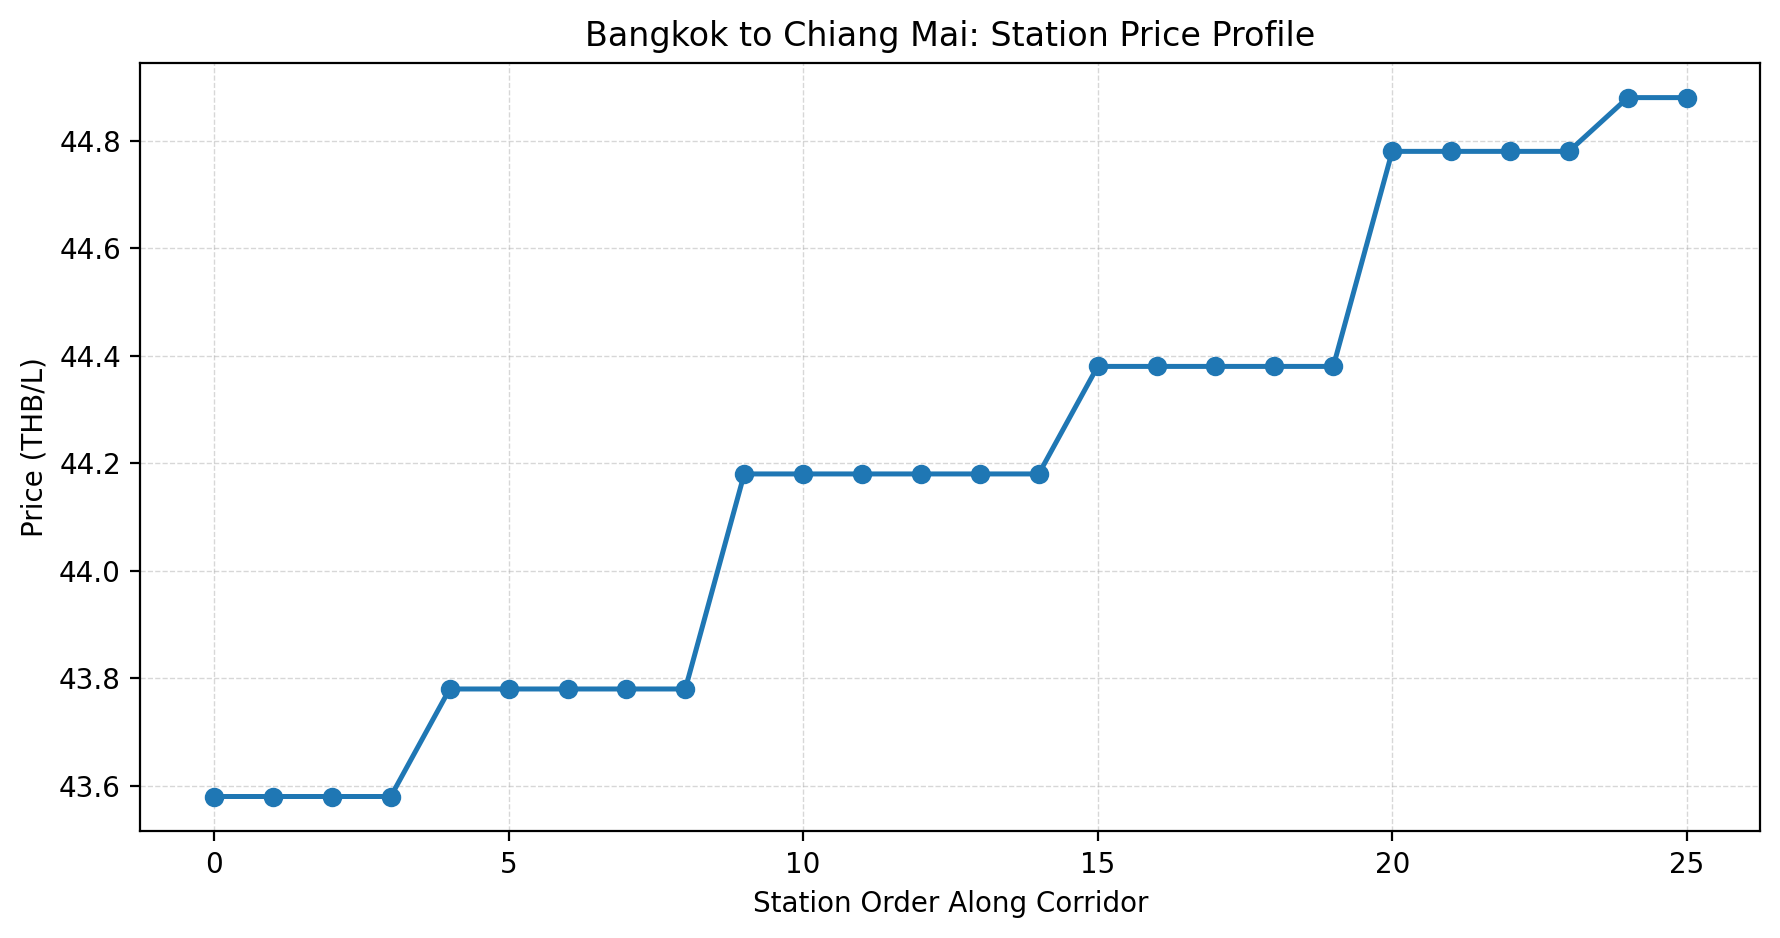
\includegraphics[width=0.88\textwidth]{../results/report_assets/exp6_real_routes/exp6_real_routes_station_prices_bkk_to_cnx.png}
      \caption{Chiang Mai price profile.}
      \label{fig:exp6_prices_cnx}
\end{figure}

\begin{figure}[H]
      \centering
      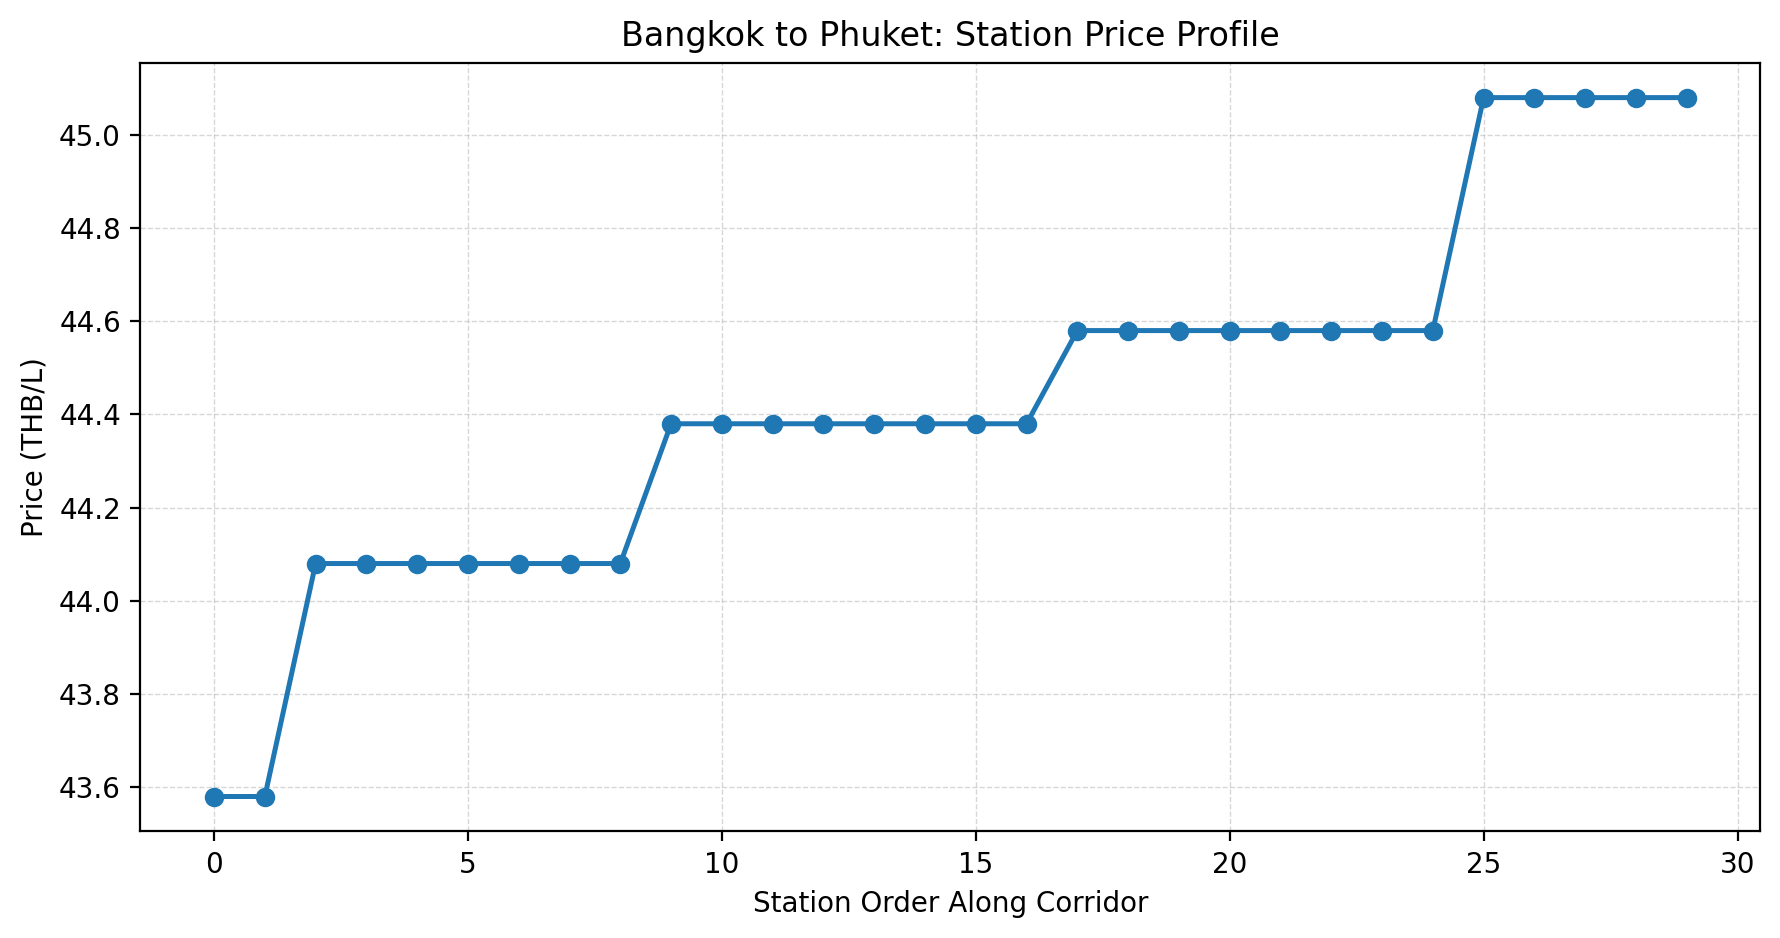
\includegraphics[width=0.88\textwidth]{../results/report_assets/exp6_real_routes/exp6_real_routes_station_prices_bkk_to_hkt.png}
      \caption{Phuket price profile.}
      \label{fig:exp6_prices_hkt}
\end{figure}

\begin{figure}[H]
      \centering
      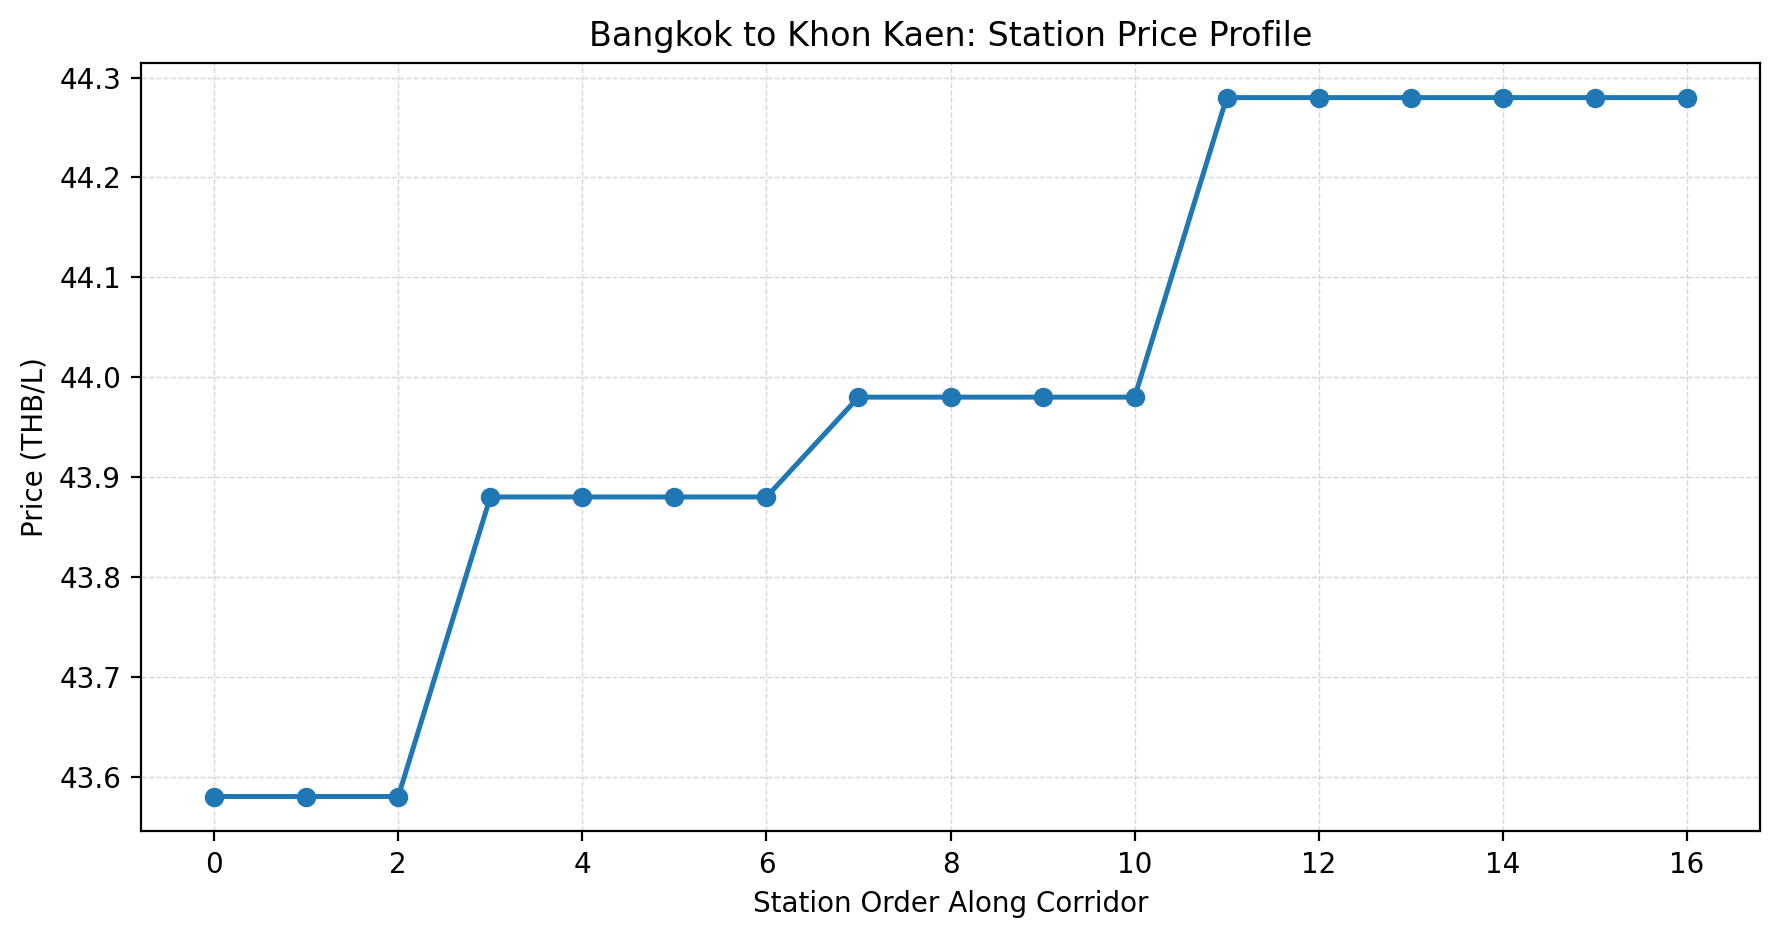
\includegraphics[width=0.88\textwidth]{../results/report_assets/exp6_real_routes/exp6_real_routes_station_prices_bkk_to_kkc.png}
      \caption{Khon Kaen price profile.}
      \label{fig:exp6_prices_kkc}
\end{figure}

\section{Limitations}

Three limitations should remain explicit in any final submission built from the current
repository snapshot.
First, the synthetic results embedded in this chapter come from the reduced 3-run profile
described in Section~\ref{sec:current_synth_snapshot} rather than the full 10{,}000-run
target profile; the full target profile has been achieved only on the real-route evaluation
(Experiment~6).
Second, the observed cost gap in Standard A* and RF-A* means that strict claims about all
four optimal algorithms agreeing on cost should not be made; the exact-agreement set in
the submitted results is Dijkstra, DP, and PF-A*, and the A*/RF-A* gap is reported as an
implementation-audit item.
Third, the current real-route dataset consists of curated corridor abstractions with
province-level prices, so Experiment~6 is discussed as a realistic corridor case study
rather than as a full raw-OSM nationwide station benchmark.
